\documentclass{article}

\usepackage{graphicx}
\usepackage{tikz}
\usepackage{tikzsymbols}
\usetikzlibrary{calc,patterns,shapes.geometric}
\pagestyle{empty}
\usepackage[margin=0pt]{geometry}
\geometry{papersize={14in,12in}}

\def\centerarc[#1](#2)(#3:#4:#5){\draw[#1] ($(#2)+({#5*cos(#3)},{#5*sin(#3)})$) arc (#3:#4:#5);}

\begin{document}
	\begin{figure}
		\centering
		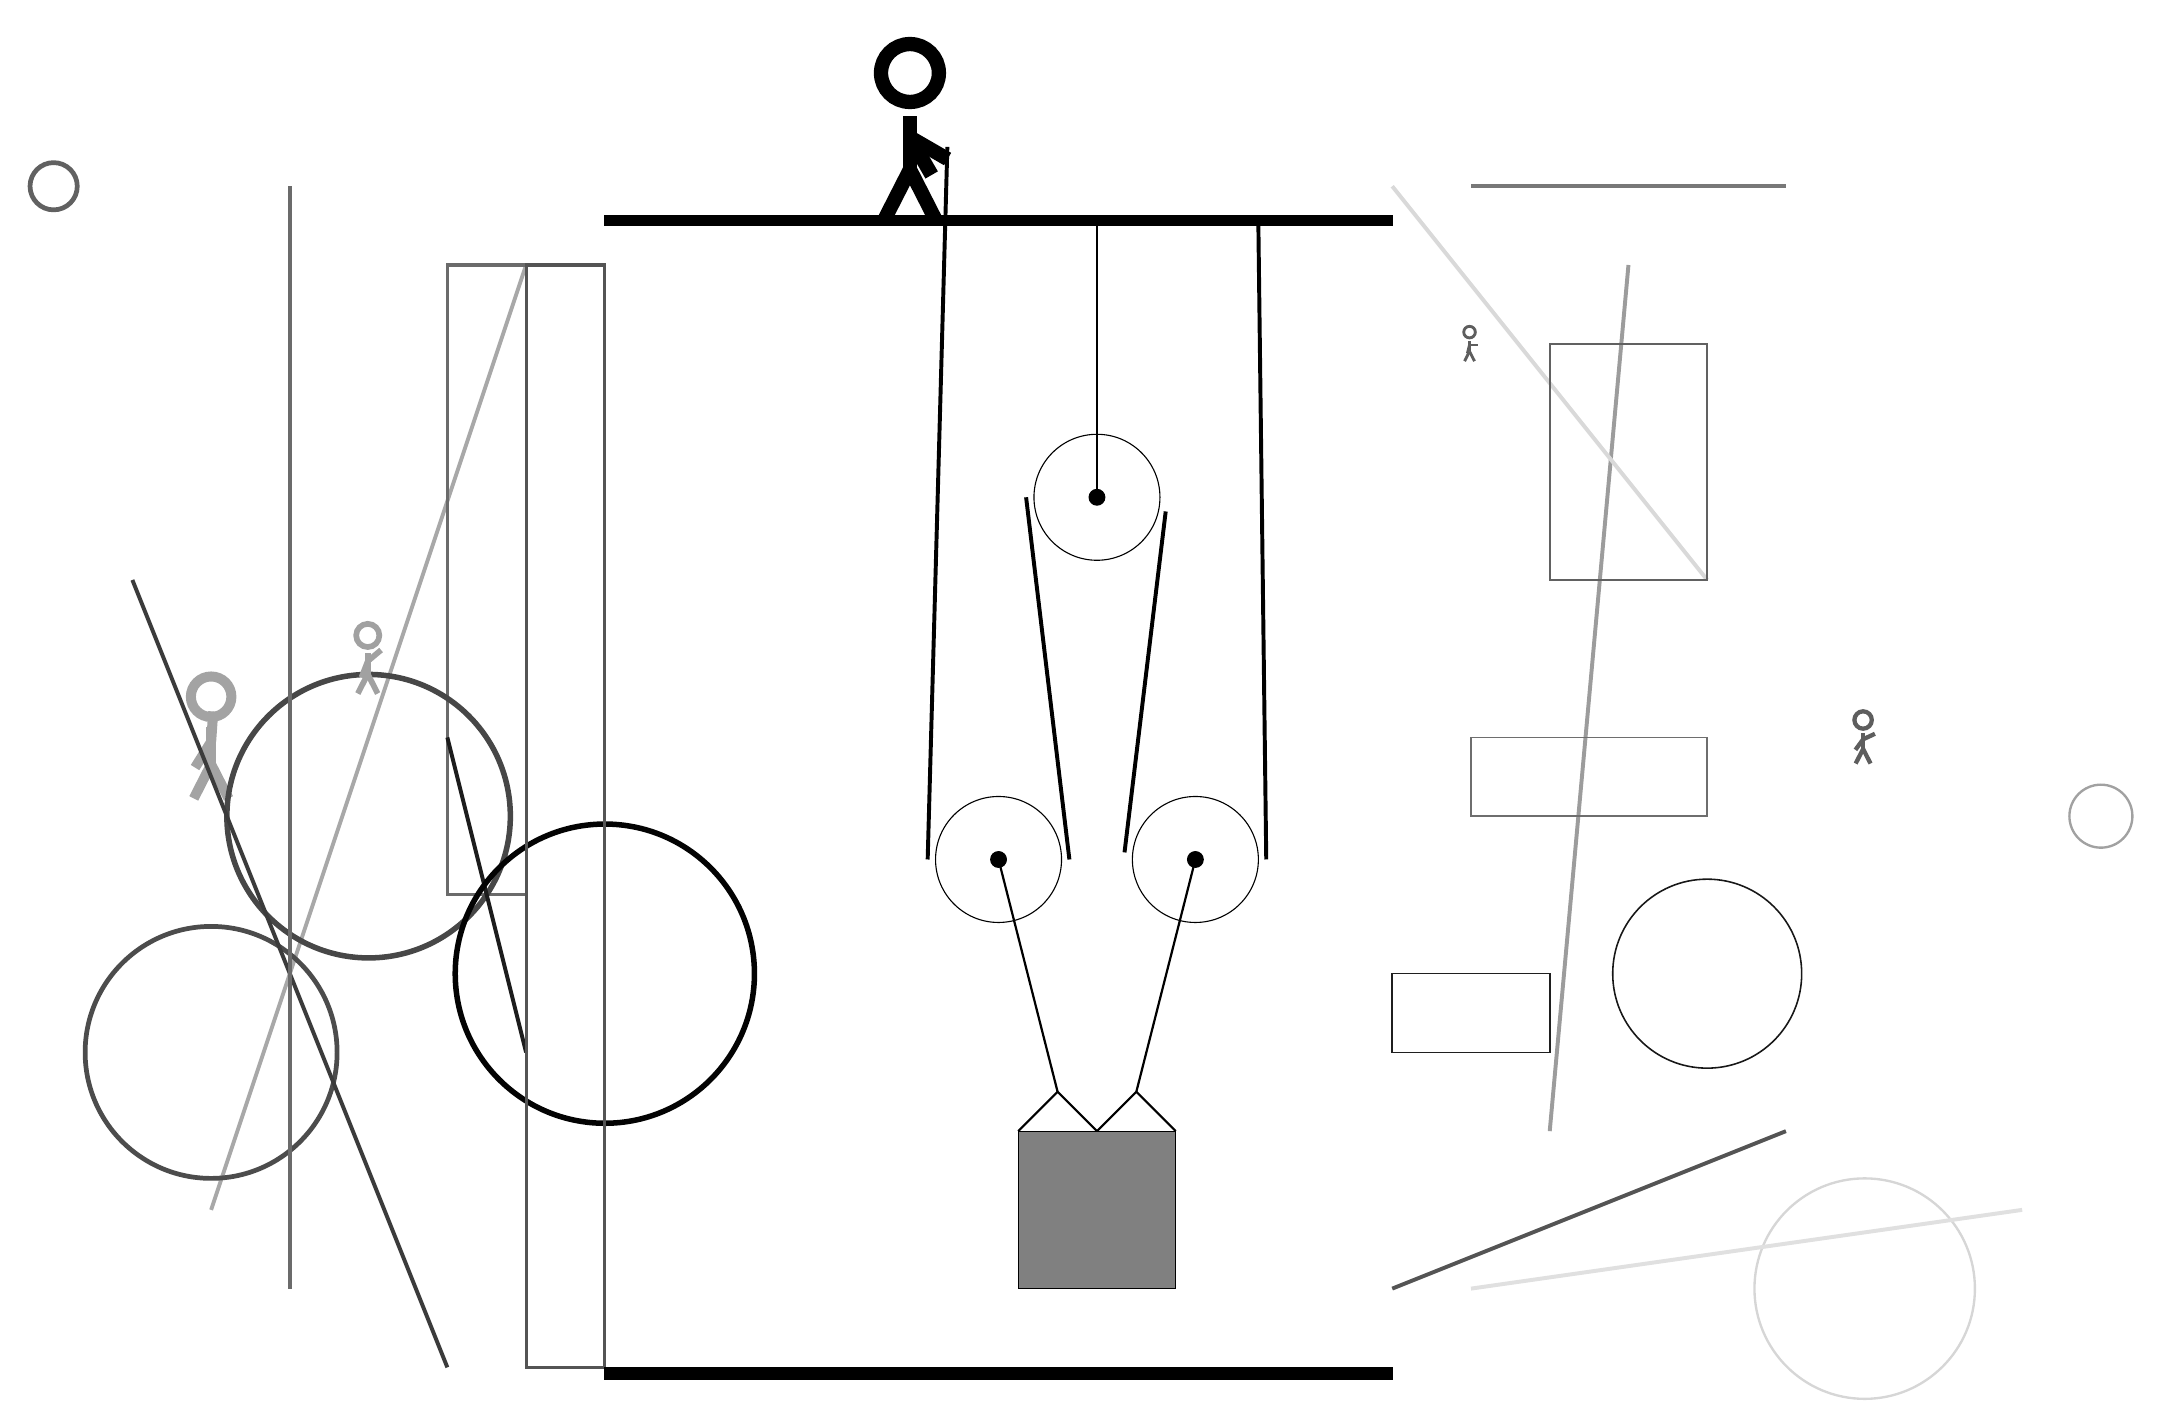
\begin{tikzpicture}
			%%%%% START %%%%%
			
			\draw[fill=black] (-4, 11.5) rectangle (6, 11.625);
			
			\draw (1, 3.45) circle (0.8);
			\draw[fill=black] (1, 3.45) circle (0.1);
			
			\draw (2.25, 8.05) circle (0.8);
			\draw[fill=black] (2.25, 8.05) circle (0.1);
			\draw[thick] (2.25, 8.05) -- (2.25, 11.5);
			
			\draw (3.5, 3.45) circle (0.8);
			\draw[fill=black] (3.5, 3.45) circle (0.1);
			
			\draw[thick] (3.5, 3.45) -- (2.75, 0.5);
			\draw[thick] (1, 3.45) -- (1.75, 0.5);
			\draw[thick]  (1.25, 0) -- (1.75, 0.5) -- (2.25, 0);
			\draw[thick]  (2.25, 0) -- (2.75, 0.5) -- (3.25, 0);
			\draw[fill=black!50] (1.25, 0) rectangle (3.25, -2);
			
			\draw[line width=0.5mm, color=black!34](-9, -1) -- (-5, 11);
			
			\draw[line width=0.4mm, color=black!58] (-5, 11) rectangle (-6, 3);
			\draw[line width=0.2mm, color=black!88] (8, 2) rectangle (6, 1);
			\draw[line width=0.5mm, color=black!67](6, -2) -- (11, 0);
			\draw [line width=0.2mm, color=black!91](10, 2) circle (1.2);
			\node[line width=0.6mm, color=black!63] at (12, 5) {\Strichmaxerl[3][54][25]};
			\node[line width=0.4mm, color=black!36] at (-9, 5) {\Strichmaxerl[7][58][86]};
			\node[line width=0.7mm, color=black!63] at (7, 10) {\Strichmaxerl[2][76][0]};
			\draw [line width=0.3mm, color=black!16](12, -2) circle (1.4);
			
			\draw [line width=0.6mm, color=black!70](-9, 1) circle (1.6);
			\draw [line width=0.7mm, color=black!72](-7, 4) circle (1.8);
			
			\draw[line width=0.5mm, color=black!12](7, -2) -- (14, -1);
			\draw[line width=0.5mm, color=black!77](-6, -3) -- (-10, 7);
			\draw[line width=0.5mm, color=black!89](-5, 1) -- (-6, 5);
			\draw[line width=0.5mm, color=black!39](9, 11) -- (8, 0);
			\draw [line width=0.6mm, color=black!62](-11, 12) circle (0.3);
			
			\draw[line width=0.5mm, color=black!15](6, 12) -- (10, 7);
			\draw [line width=0.7mm, color=black!99](-4, 2) circle (1.9);
			\draw[line width=0.2mm, color=black!57] (7, 5) rectangle (10, 4);
			\node[line width=0.3mm, color=black!37] at (-7, 6) {\Strichmaxerl[4][69][40]};
			\draw[line width=0.5mm, color=black!53](11, 12) -- (7, 12);
			
			\draw [line width=0.3mm, color=black!37](15, 4) circle (0.4);
			
			\draw[line width=0.2mm, color=black!62] (8, 10) rectangle (10, 7);
			\draw[line width=0.4mm, color=black!67] (-4, -3) rectangle (-5, 11);
			\draw[line width=0.5mm, color=black!58](-8, 12) -- (-8, -2);
			
			
			\draw[line width=0.5mm] (0.35, 12.5) --  (0.1, 3.45);
			\centerarc[line width=0.5mm](1, 3.45)(180:360:0.9);
			\draw[line width=0.5mm] (1.9, 3.45) -- (1.35, 8.05);
			\centerarc[line width=0.5mm](2.25, 8.05)(-20:180:0.9);
			\draw[line width=0.5mm](3.123, 7.87) -- (2.6, 3.54);
			\centerarc[line width=0.5mm](3.5, 3.45)(160:360:0.9);
			\draw[line width=0.5mm](4.4, 3.45) -- (4.3, 11.5);
			
			\node at (-0.07, 12.7) {\Strichmaxerl[10][120][-30]};
			
			\draw[fill=black] (-4, -3) rectangle (6, -3.15);
			
			%%%%% END %%%%%
		\end{tikzpicture}
	\end{figure}	
\end{document}